
\documentclass{article}
\usepackage[english]{babel}
\usepackage[margin=1in]{geometry}
\usepackage{multicol}
\usepackage{background}
\usepackage[math]{blindtext}% just to generate filler text
\usepackage{amsmath}
\usepackage{algorithm}
\usepackage[noend]{algpseudocode}
\usepackage{subfigure}
\usepackage{graphicx}
\usepackage{natbib}
\usepackage{parskip}
\usepackage{graphicx}

\graphicspath{ {images/} }
\newtheorem{theorem}{Theorem}
\usetikzlibrary{calc}
\SetBgScale{4}
\SetBgColor{gray}
\SetBgAngle{90}
\SetBgContents{arXiv: some other text goes here}
\SetBgPosition{-1.5,-10}

%opening
%\title{Efficient Computation of Abelian Sandpiles Exploiting Dhar's Spanning Tree Bijection}
\date{\vspace{-5ex}}

%%%STYLES FOR DHAR LATTICE

\tikzstyle myBG=[line width=3pt,opacity=1.0]
\tikzstyle{vertex}=[circle, fill=gray, draw, inner sep=0pt, minimum size=10pt]
\tikzstyle{vertexLight}=[circle, fill=white, draw, inner sep=0pt, minimum size=10pt]
\newcommand{\vertex}{\node[vertex]}
\newcommand{\vertexLight}{\node[vertexLight]}
\newcommand{\drawLinewithBG}[2]
{
	\draw[black] (#1) -- (#2);
}
\newcommand{\grid}[3]
{
	\begin{scope}      
		\draw [#3,step=2cm] grid (6,6);
	\end{scope}
}
%%%%%%%%%%%%%%%%%%%%%%%%%%

\tikzset{darkstyle/.style={draw}}
\usetikzlibrary{plotmarks}
\usetikzlibrary{shapes,snakes}

\bibliographystyle{abbrvnat}

\begin{document}

{\centering
	{\bfseries\Large Numerics of the Branching Wiener Sausage\bigskip}	
	\\S Amarteifio,...
		 \\
		\normalfont (Dated: November 1, 2016)	
	
}



\begin{abstract}
The C code can be used to run the Branching Wiener Sausage process for different systems sizes, number of dimensions and boundary conditions. Details of the process and specifics about simulation are described.
\end{abstract}

\begin{multicols}{2}
	% the article contents goes here

\section{Overview}

The BWS process is a branching and diffusion process. Any particle either hops (diffuses) with probability $h$, branches with probability $\sigma$ or becomes extinct with probability $\epsilon$. The critical branching rate is given; we fix $\sigma=\epsilon$. In the current implementation parameters are chosen such that $h+\sigma+\epsilon=1$ and $h$ is chosen to be high e.g. $0.95$. Each of these sub processes is a \textit{Poisson} process. As the system evolves, an exponential waiting time for an event is simulated as $-\ln(1-U)/N$ where $U\sim U(0,1)$ and $N$ is the size of the population. Time is stored as a \verb|long double|. The process is \textit{bosonic}. When branching occurs, offspring are added \textit{locally} i.e. to the same site as the parent. \\
Typically we choose system sizes of powers of 2 (specifically $2^n - 1$) starting from $2^4 - 1$. We choose an upper bound that accounts for memory usage for higher dimensions. For example, two dimensions can easily exceed $2^10$ while three and five dimensions may struggle depending on the implementation and the hardware.
\\

\subsection{Lattice \& Boundary Conditions}

The $D$ dimensional lattice is mapped to a one dimensional data structure using a suitable mapping $f: \mathcal{R}^D\to \mathcal{R}$, specifically we use
\begin{equation}
f(x_0, x_1,..., x_d) = \sum_{d=0}^{D-1} x_d L^d
\end{equation}
With this mapping, a particle that hops $1$ site in any direction in $\mathcal{R}^D$ jumps $\pm L^d$ in $R^1$ for a given component axis\footnote{Conventionally we assign even numbers in $2D$ to positive(forward) moves and odd numbers to negative (back) moves}. \\
The boundary conditions are enforced by creating a function that maps each site to a \textit{partition} of the space. This function, $g$, maps a site $i$ to a partition in the context of some axis/dimension $d$. Simply, $g(i,d)=floor(i/L^{d+1})$. It is illegal for a particle to hop between partitions\footnote{TODO: Performance hint to predetermine boundary sites with lattice flags to avoid checking partitions each time. }. When a jump is computed along an axis such that $i'= i + L^d$, we can check the condition $g(i,d)\stackrel{?}{=}g(i',d)$.
\\
A bitmask is used to close boundaries on given axes. For example setting bits $0,1$ closes the first component axis at both ends to create a toroidal axis (as opposed to closed/reflecting boundaries).


\subsection{Exponents for 2D}
Considering various boundary conditions for various system sizes, we study behaviour in a region dominated by system size or extinction. There is a certain upper regime where \textit{distinct sites visited} is dominated by extinction. For small systems, the boundary conditions dominate. Looking at the first moment for a number of system sizes, one can see that there is a region where, independent of system size, the observable grows with \textit{t} (power law).


\begin{center}
	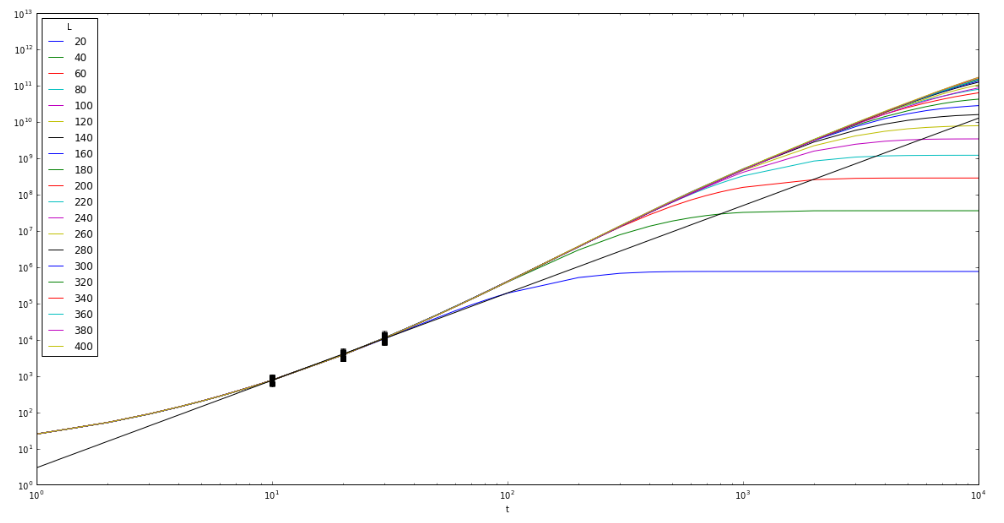
\includegraphics[scale=0.3]{sample1}
\end{center}


The first eight moments are shown for a system of size 100

\begin{center}
	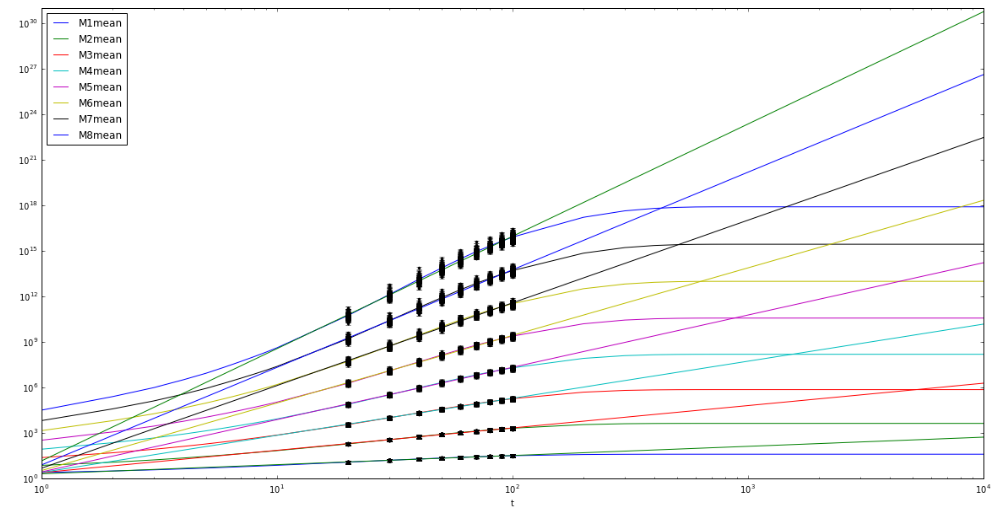
\includegraphics[scale=0.3]{sample2}
\end{center}


\begin{center}\begin{tabular}
		{|c|c|c|c|}
		\hline
		\textbf{Amp} & \textbf{Index} & \textbf{Moment n=} & \textbf{$\Delta$ Index}
		\\
		\hline
		2.82 & 0.58 & 1.00 & nan
		\\
		1.04 & 1.77 & 2.00 & 1.18
		\\
		0.39 & 3.02 & 3.00 & 1.25
		\\
		0.19 & 4.27 & 4.00 & 1.24
		\\
		0.11 & 5.49 & 5.00 & 1.23
		\\
		0.09 & 6.70 & 6.00 & 1.21
		\\
		0.07 & 7.89 & 7.00 & 1.19
		\\
		0.07 & 9.07 & 8.00 & 1.18
		\\
		\hline
	\end{tabular}\end{center}
	
	For 2D (open boundaries) the table shows the exponents. 

\subsection{Exponents for 3D}

The first eight moments are shown for a system of size 100

\begin{center}
	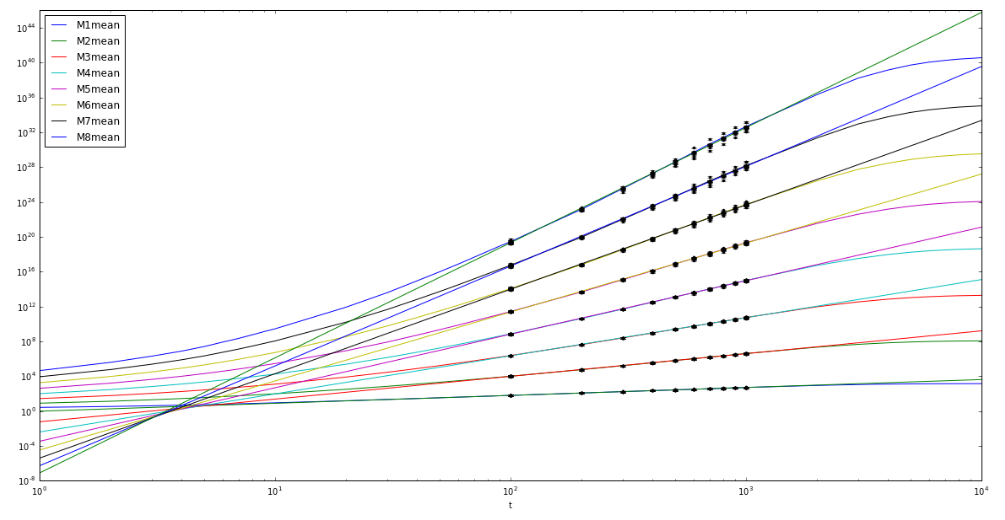
\includegraphics[scale=0.3]{3d_sample}
\end{center}

\begin{center}\begin{tabular}
		{|c|c|c|c|}
		\hline
		\textbf{Amp} & \textbf{Index} & \textbf{Moment n=} & \textbf{$\Delta$ Index}
		\\
		\hline
		1.00 & 0.91 & 1.00 & nan
		\\
		0.06 & 2.61 & 2.00 & 1.70
		\\
		0.00 & 4.37 & 3.00 & 1.76
		\\
		0.00 & 6.14 & 4.00 & 1.77
		\\
		0.00 & 7.92 & 5.00 & 1.77
		\\
		0.00 & 9.69 & 6.00 & 1.77
		\\
		0.00 & 11.46 & 7.00 & 1.77
		\\
		0.00 & 13.22 & 8.00 & 1.76
		\\
		\hline
	\end{tabular}\end{center}
%\bibliography{document}

\subsection{Exponents for 5D}

The first eight moments are shown for a system of size 100

\begin{center}
	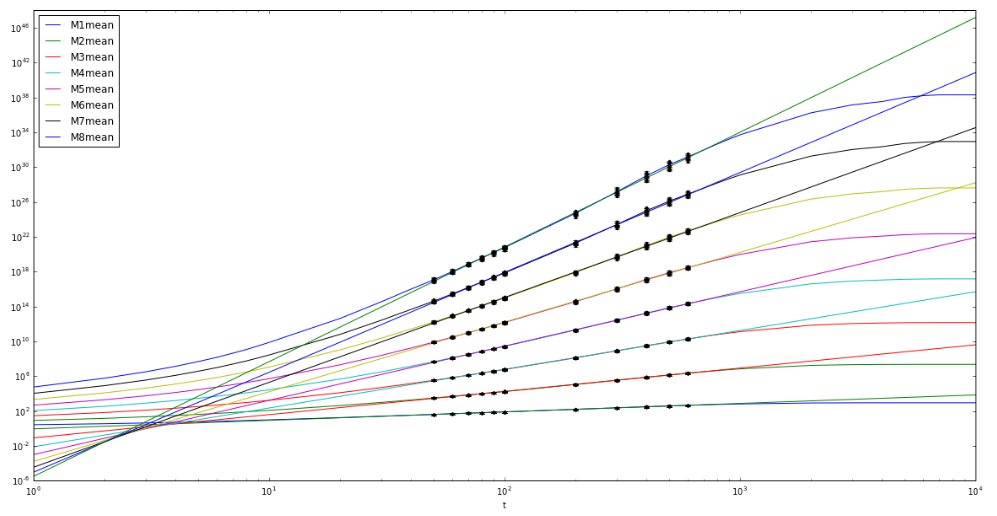
\includegraphics[scale=0.3]{5d_sample}
\end{center}

\begin{center}\begin{tabular}
		{|c|c|c|c|}
		\hline
		\textbf{Amp} & \textbf{Index} & \textbf{Moment n=} & \textbf{$\Delta$ Index}
		\\
		\hline
		0.94 & 0.97 & 1.00 & nan
		\\
		0.09 & 2.67 & 2.00 & 1.70
		\\
		0.01 & 4.45 & 3.00 & 1.78
		\\
		0.00 & 6.23 & 4.00 & 1.78
		\\
		0.00 & 8.00 & 5.00 & 1.77
		\\
		0.00 & 9.75 & 6.00 & 1.75
		\\
		0.00 & 11.47 & 7.00 & 1.72
		\\
		0.00 & 13.17 & 8.00 & 1.70
		\\
		\hline
	\end{tabular}\end{center}
 
\end{multicols}



\end{document}
